\documentclass[11pt, a4paper]{article}
\usepackage{url}
\usepackage{anyfontsize} 
\usepackage{setspace}     
\usepackage{hyperref}		
\usepackage[misc]{ifsym}
\usepackage{graphicx}
\usepackage{changepage}
\usepackage{amsmath}
\usepackage[]{algorithm2e}
\usepackage{pdfpages}


\SetKwProg{Fn}{Function}{}{}
\title{Multiplication \\of two digit numbers}
\author{Sonam Tenzin}
\date{6th March 2017}

\begin{document}
	\maketitle
	\newpage
	\section{\underline{Case 1}}
	\subsection{Explanation}
	The first digits are same, and the last ones add up to 10. wdasdladkjad hafohlidfnja afnjihalj fnaljnlsanflj  fjajfjasf The first digits are same, and the last ones add up to 10. wdasdladkjad hafohlidfnja afnjihalj fnaljnlsanflj  fjajfjasf The first digits are same, and the last ones add up to 10. wdasdladkjad hafohlidfnja afnjihalj fnaljnlsanflj  fjajfjasf The first digits are same, and the last ones add up to 10. wdasdladkjad hafohlidfnja afnjihalj fnaljnlsanflj  fjajfjasf
	The first digits are same, and the last ones add up to 10. wdasdladkjad hafohlidfnja afnjihalj fnaljnlsanflj  fjajfjasf
	The first digits are same, and the last ones add up to 10. wdasdladkjad hafohlidfnja afnjihalj fnaljnlsanflj  fjajfjasf
	Suppose we want to calculate $66 \times 64$.\footnote{graphical explanation next page}\\
	

	{\begin{center}
	\begin{tabular}{rl}
		64 & 66\\
		\hline
		 6$\times$(6+1) & 6$\times$4\\
		 42 & 24\\
		 
	\end{tabular}
	\end{center}}
	Ans : 4224
		
	\subsection{Pseudocode}\label{B1}
	\begin{algorithm}
		{\Fn{(number1,number2)}{
		a $=$ ten's digit(number1)\\
		b $=$ a $\times$ (a+1)\\
		c $=$ Multiply unit digits\\
		ans $=$ 100b + c\\
		\textbf{return} ans\\
		}}
	\end{algorithm}
		
	\subsection{Proof of Correctness:\label{C1}\\}
	Let the numbers be m and n
	\begin{align*}
		m &= 10x+y\\%\label{1}
		n &= 10x+10-y\\%\label{eq:2}
	\end{align*}
	the result of their multiplication is given by:\\
	\begin{align*}
		ans &= m \times n\\
				&= (10x+y) \times (10x +10-y)\\
				&= 100x(x+1) + y(10-y) 
	\end{align*}
	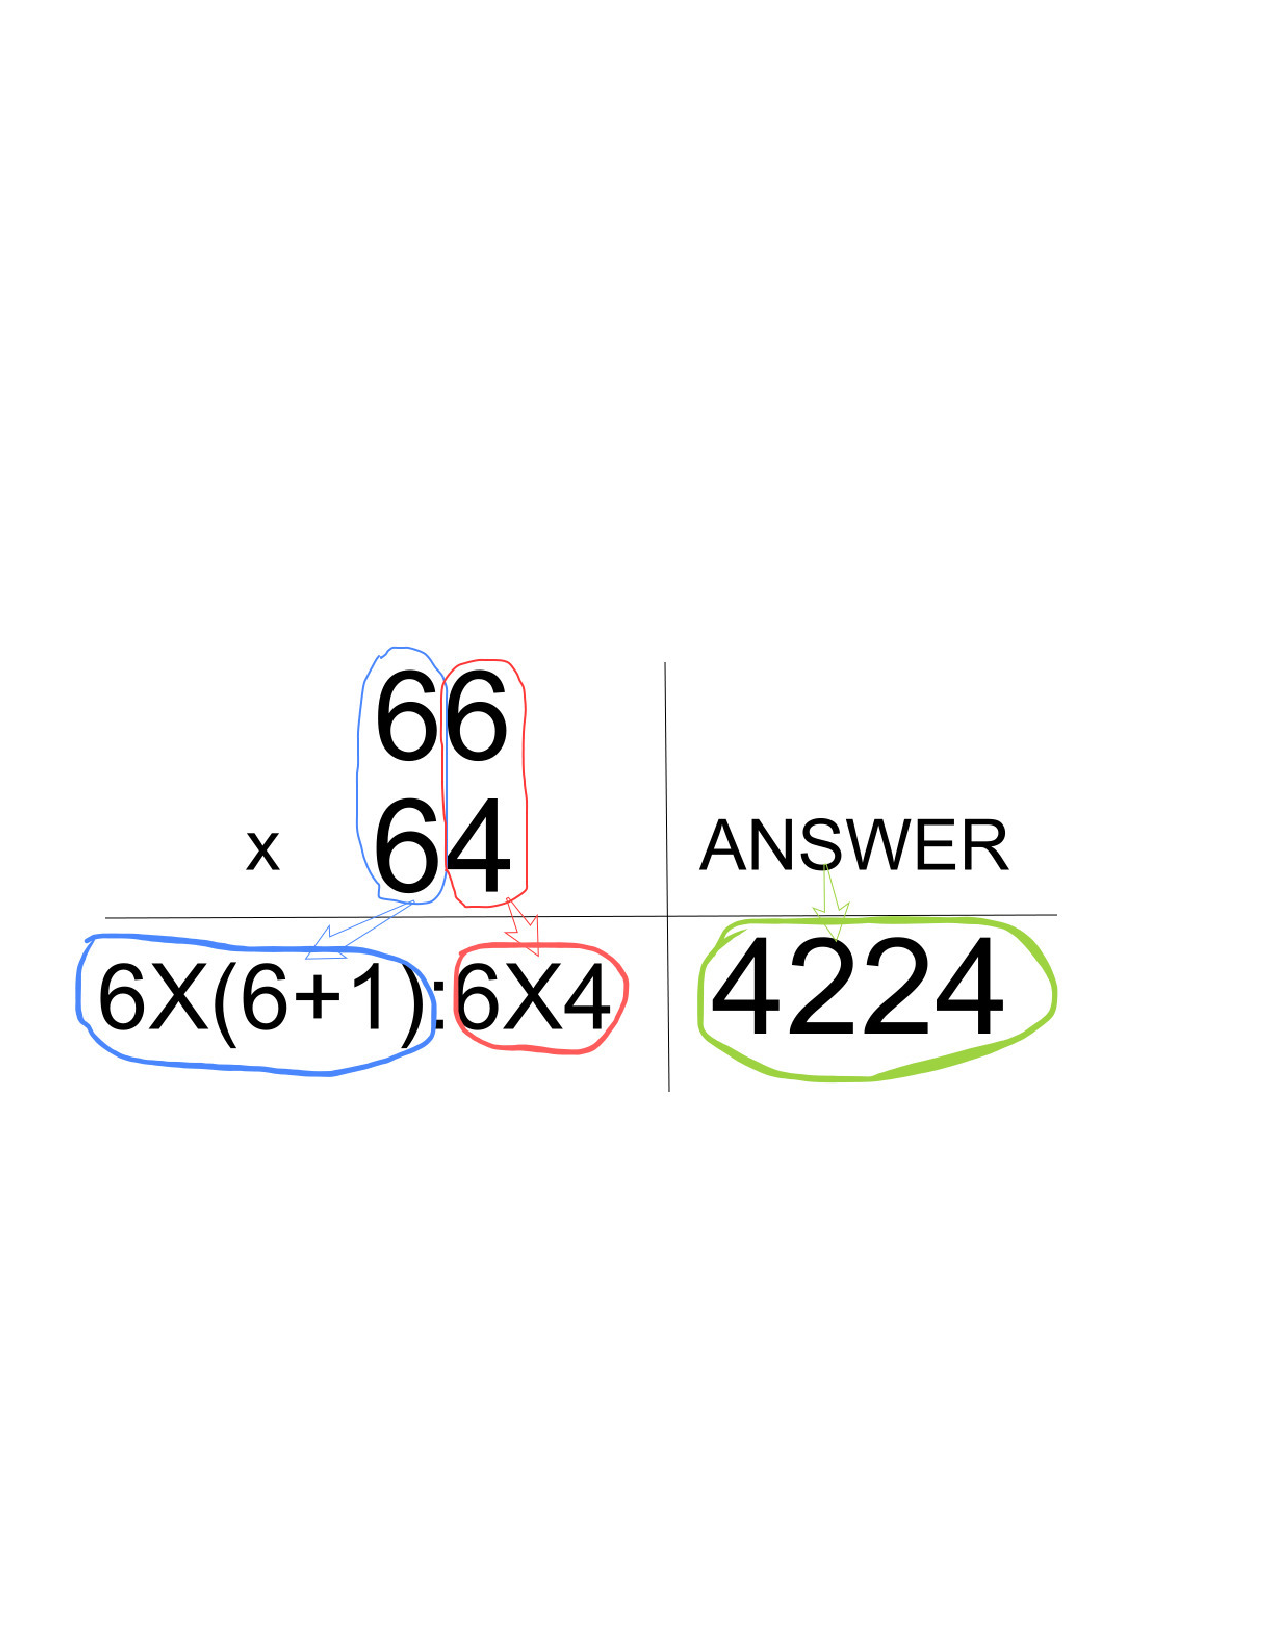
\includepdf{1}
	
	\newpage
	\section{\underline{Case 2}}
	\subsection{Explanation}
	The first digits add up to 10, and the last ones are same.
	Suppose we want to calculate $34 \times 74$.
	
	{\begin{center}
	\begin{tabular}{rl}
		34 & 74\\
		\hline
		 3$\times$7+4 & 4$\times$4\\
		 25 & 16\\
	\end{tabular}
	\end{center}}
	Ans = 2516
	
	\subsection{Pseudocode}\label{B2}
	\begin{algorithm}
		{\Fn{(number1,number2)}{
		a $=$ ten's digit(number1)\\
		b $=$ ten's digit(number2)\\
		c $=$ a $\times$ b + unit digit\\
		d $=$ square of unit digit\\
		ans $=$ 100c + d\\
		\textbf{return} ans
		}}
	\end{algorithm}
	
	\subsection{Proof of Correctness:\label{C2}\\}
	Let the numbers be m and n
	\begin{align*}
		m &= 10x+y\\
		n &= 10(10-x)+y\\
				&= 100 - 10x +y
	\end{align*}
	the result of their multiplication is given by:\\
	\begin{align*}
		ans &= number1 \times number2\\
				&= (10x+y) \times (100 - 10x + y)\\
				&= 100\{x(10-x)+y\} + y^2
	\end{align*}
	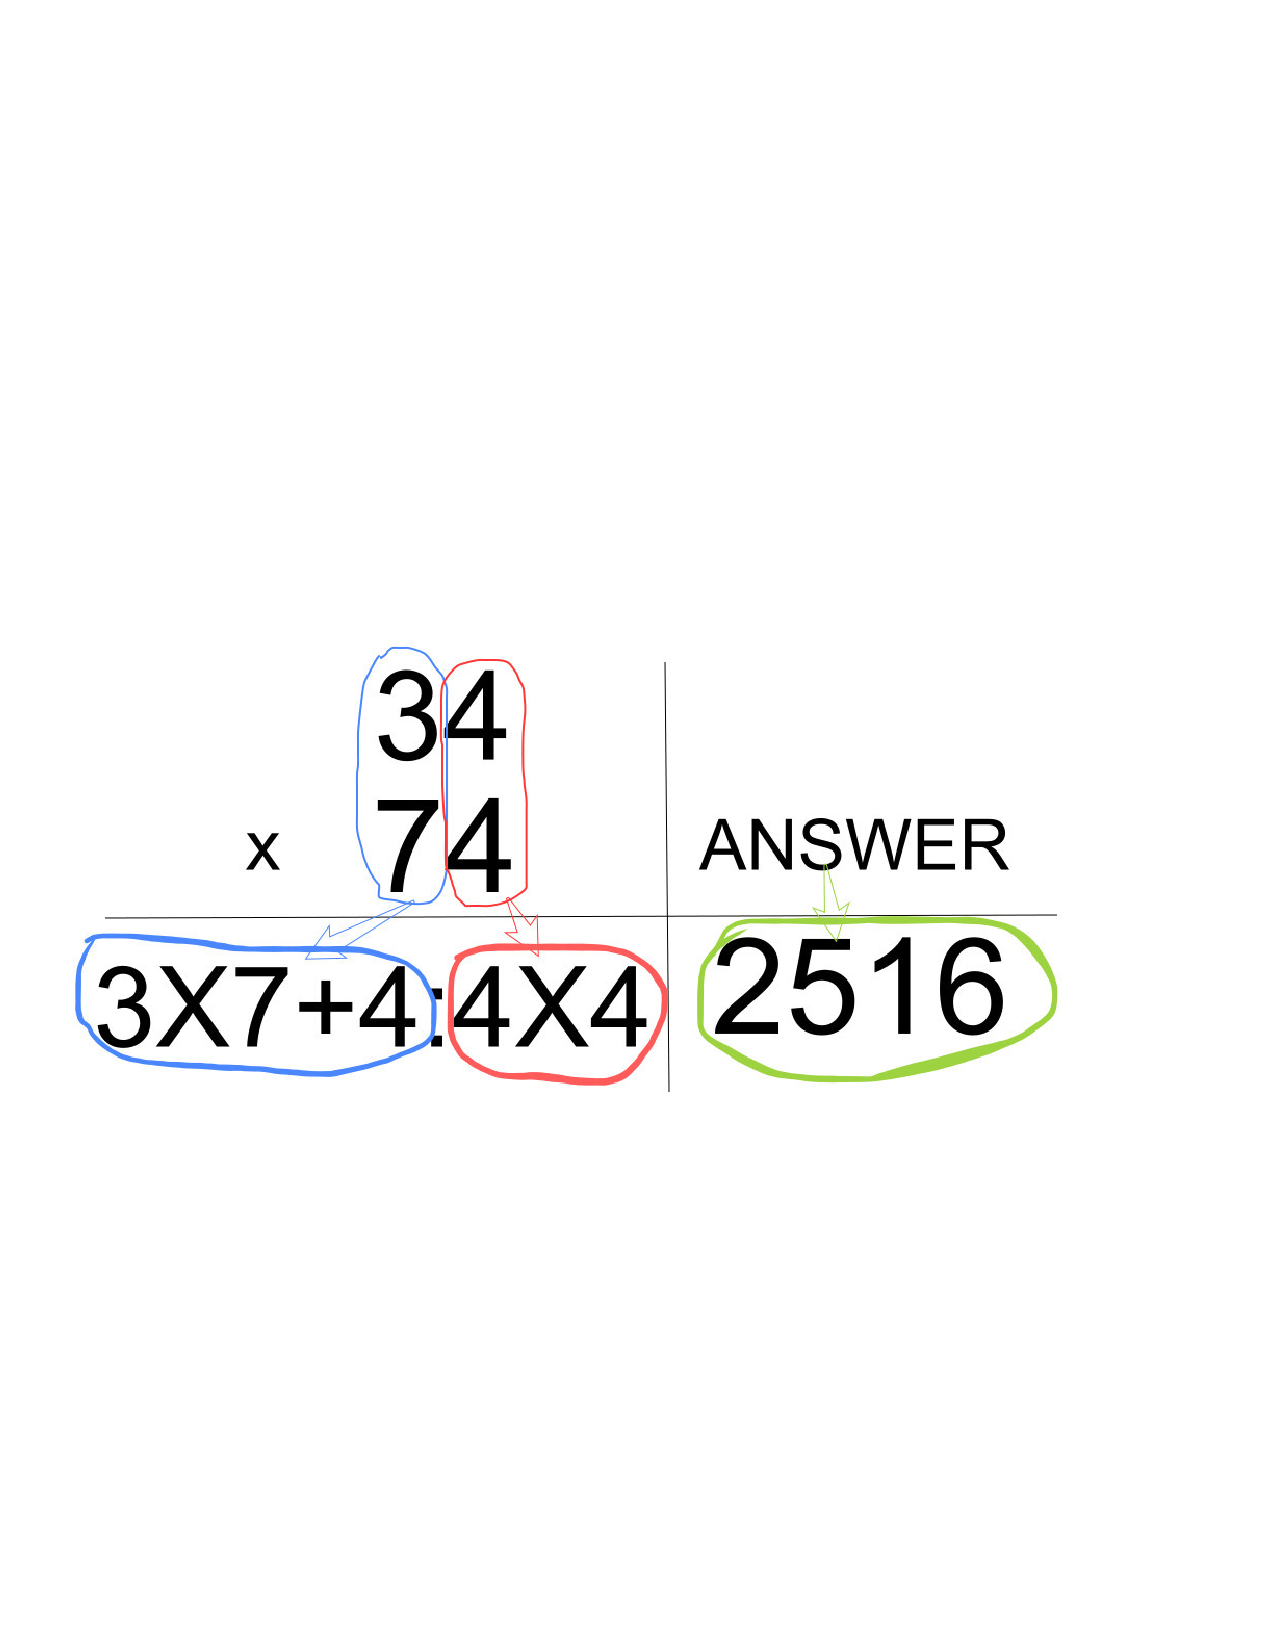
\includepdf{2}
	
	% pdflatex a.tex
	% bibtex a.aux
	\newpage
	\vspace{0.5cm}
	\hspace{-0.7cm}
	In case you want more on the subject of fast multiplications, check \textit{Avsijbv}
	\cite{cite1}\\
	For the complete code mentioned in \ref{B1} and \ref{B2} check \url{http://jkafjuyaf.com/jggosj/}
	\bibliographystyle{plain}
	\bibliography{bib1}
	
\end{document}

